\documentclass[10pt,a4paper]{article}
\usepackage[margin=17mm]{geometry}
\usepackage[T1]{fontenc}
\usepackage{newtxtext,newtxmath}
\usepackage{microtype,graphicx,booktabs,caption,xcolor,hyperref}
\hypersetup{colorlinks=true,urlcolor=teal,linkcolor=black,
pdftitle={Visual preprocessing, sparse codes and navigation accuracy},
pdfsubject={Expanded ApiaViz study: matched navigation baselines and component tests}}
\graphicspath{{figures/}}
\setlength{\parindent}{0pt}
\setlength{\parskip}{4pt}
\captionsetup{font=small,labelfont=bf,skip=3pt,hypcap=false}
\newcommand{\topic}[1]{\vspace{4pt}{\large\bfseries #1}\par}
\begin{document}
{\LARGE\bfseries Visual preprocessing, sparse codes\par
and navigation accuracy\par}
\vspace{3pt}
{\small Expanded ApiaViz simulation study\hfill 29 September 2026}
\vspace{5pt}\hrule\vspace{4pt}

{\small\textbf{Abstract.} We tested whether fixed insect-inspired visual
processing improves autonomous navigation through a spiking representation.
An expanded comparison of 440 trials did not reproduce the accuracy advantage
seen in a four-route pilot. ApiaViz and Sobel plus colour each completed 29 of
40 trials; their mean deviations were 55.2 and 50.4\,cm. No baseline comparison
was significant after multiple-comparison correction. Component tests show
that local adaptation makes different places more distinguishable, but this
does not establish superior navigation. Both frontends often preserve a heading
parallel to the route without steering back towards it.\par}

\topic{1\quad Matched learning and navigation}
Insect mushroom bodies learn associations using sparse activity in Kenyon
cells (KCs). Ardin et al.~[1] applied this principle to route memory;
Gattaux et al.~[2] combined Sobel filtering with directional memories and
robot control. We compare their associated input operations within one shared
navigation model, rather than reproducing either complete published system.

Eight approximately 8\,m routes in one synthetic grassland were tested with
five fixed wiring seeds. Six baselines and five component interventions gave
$8\times5\times11=440$ trials. All conditions learned the same nine lateral
views spanning $\pm20$\,cm every 10\,cm along a route, facing its local tangent.
Only image processing changed. Five maps entered the same pooling,
standardisation, fixed random projections, 8,000 leaky integrate-and-fire KCs,
binary spike-overlap memory and controller. Visual filters were untrained;
route acquisition stored the memories. Spike timing had 1\,ms resolution.

The agent scanned 13 headings across $\pm60^\circ$, moved 10\,cm towards the
most familiar, and stopped within 20\,cm of the nest or after 200 steps.
There were no corrective resets. This is the project's ``open-loop'' condition:
visual feedback remains available. The eight routes exclude the four-route
matched pilot but are not an entirely unexamined project test set.

\topic{2\quad The pilot advantage did not replicate}
\begin{center}
\small
\begin{tabular}{lrrrr}
\toprule
Input & Completed & Deviation (cm) & Difference (cm) & Holm $p$\\
\midrule
ApiaViz & 29/40 & 55.2 & --- & ---\\
Grayscale & 25/40 & 63.4 & $+8.2$ & 1.000\\
Raw colour & 26/40 & 38.0 & $-17.2$ & 1.000\\
Simple opponency & 27/40 & 69.9 & $+14.7$ & 1.000\\
Sobel + colour & 29/40 & 50.4 & $-4.8$ & 1.000\\
Ardin-style input & 6/40 & 104.7 & $+49.5$ & 0.195\\
\bottomrule
\end{tabular}
\end{center}
\vspace{-4pt}
{\small Mean deviation includes failures. Positive differences favour ApiaViz.
Ardin-style input uses inversion, local equalisation and $10\times36$
downsampling within the shared model.\par}

\begin{center}
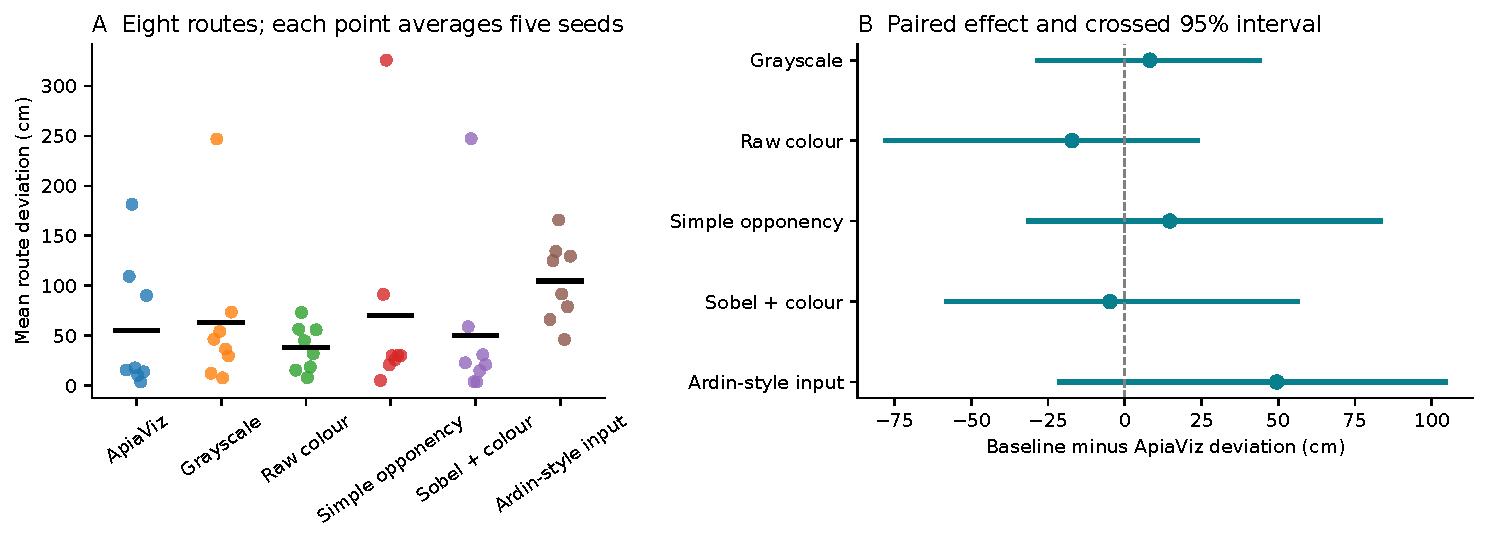
\includegraphics[width=.96\linewidth]{navigation.pdf}
\captionof{figure}{\textbf{Navigation varies substantially across routes and seeds.}
Each point averages five seeds on one route. Intervals resample both routes
and seeds; all include zero. They are unadjusted 95\% intervals.}
\end{center}

\newpage
\topic{2\quad Uncertainty and sensitivity}
The primary endpoint was mean distance to the nearest taught route sample
over the entire run. The protocol was fixed before inspecting these outcomes.
Five seeds were averaged within each route; two-sided sign-flip tests enumerated
all 256 sign assignments of the eight route differences. Holm correction covered
the five baseline comparisons. These tests assume exchangeable signs under the
null and condition on the chosen seeds. Steps and probe images were not treated
as independent replicates. Crossed bootstrap intervals used 20,000 resamples
of both routes and seeds~[5]. All inference remains conditional on one world.

For Sobel minus ApiaViz, the mean difference was $-4.8$\,cm with a crossed
95\% interval of $[-58.2,+56.2]$\,cm. Seed-specific differences ranged from
$-65.9$ to $+51.0$\,cm. The interval is too wide to establish either superiority
or equivalence. Ardin-style input had an unadjusted $p=0.039$, which became
$p=0.195$ after correction.

Long excursions raise the average error, but the early trajectory does not
restore the pilot result: mean continuous-route error over the first 50 steps
was 16.1\,cm for ApiaViz, 15.5\,cm for Sobel and 13.9\,cm for raw colour.
Prespecified secondary analyses using the continuous route or median deviation
also gave no significant corrected baseline comparison.

\topic{3\quad What changes inside the representation?}
\begin{center}
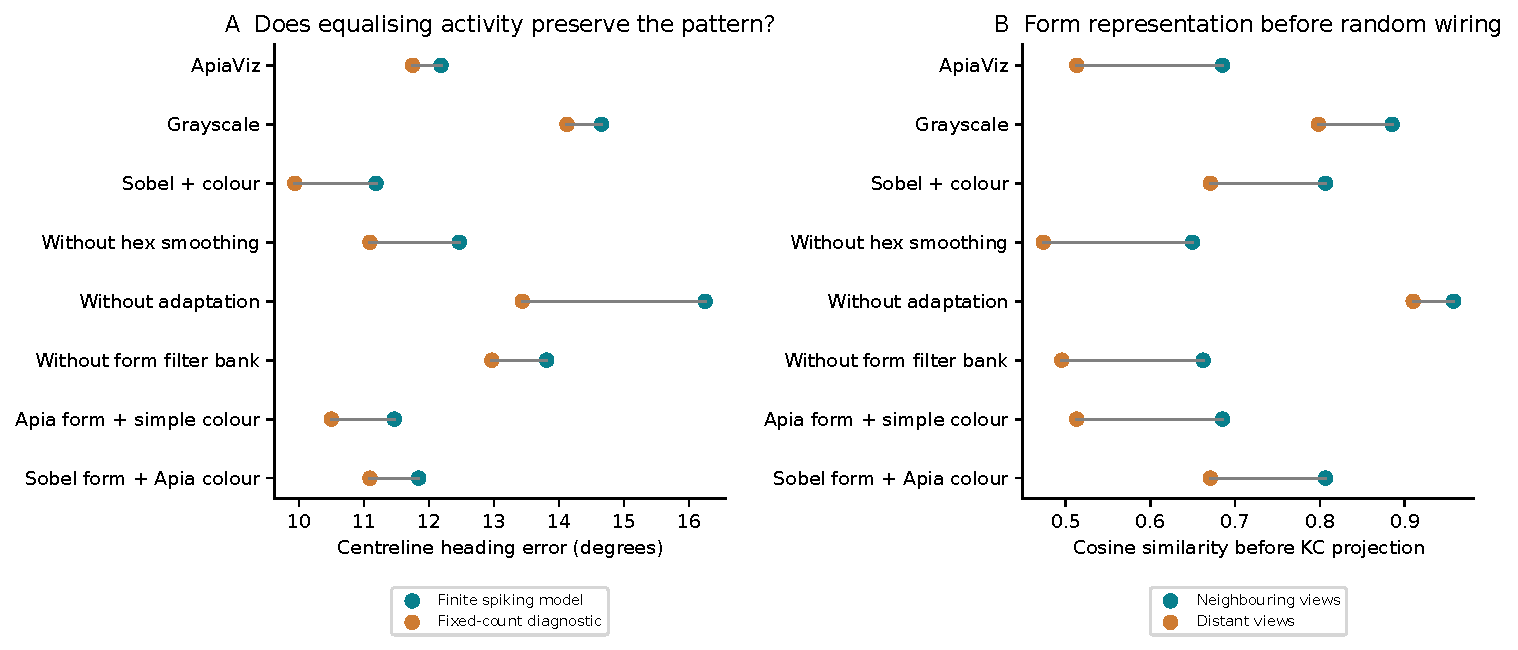
\includegraphics[width=\linewidth]{controls.pdf}
\captionof{figure}{\textbf{Different representations remain different at equal activity.}
The offline diagnostic selects exactly 5\% of cells per stream from continuous
drives, also removing finite timing. The right panel measures form-feature
similarity before random wiring. These are descriptive probe results.}
\end{center}

\textbf{Local adaptation reduces ambiguity between places.}
Removing adaptation raised distant-view form similarity from 0.513 to 0.910
before projection. Effective dimensionality fell from 25.8 to 9.9, indicating
less varied features. After spike generation, distant-view overlap rose from
0.432 to 0.611 and centreline heading error increased from $12.2^\circ$ to
$16.3^\circ$. This agrees with examining how visual similarity translates
into KC recruitment~[3]. Nevertheless, the navigation effect of removing
adaptation was uncertain: $+19.6$\,cm, adjusted $p=0.719$.

\textbf{Smoothing trades discrimination for continuity.}
Removing hexagonal averaging reduced overlap for neighbouring views
(0.552 to 0.495) and distant views (0.432 to 0.384). Processed colour also
increased similarity at both distances. Neither smoothing removal nor either
colour-pathway exchange gave a significant corrected navigation effect.

\textbf{The form pathway is dominated by smoothed local contrast.}
About 90\% of its standardised squared feature magnitude lay in the smoothed,
adapted channel, rather than the two ON/OFF channels. This is not a causal
importance estimate. The filter-bank intervention removed all three filters,
so it cannot isolate a benefit of centre--surround inhibition.

\newpage
\topic{4\quad Sparse activity does not guarantee useful steering}
We tested identical images at eight positions halfway between teaching samples,
five lateral offsets and 13 headings, both clean and at 60\% brightness.
These common-pose tests produced 35,200 decisions across the main conditions.
They separate representation differences from differences in travelled paths.

ApiaViz and Sobel activated 4.92\% and 5.08\% of KCs on average. Equalising
the activity count in 440 additional offline conditions did not reverse their
heading-error ranking: ApiaViz gave $11.8^\circ$, Sobel $9.9^\circ$, and ApiaViz
without adaptation $13.4^\circ$. Thus local discrimination differences persist
at equal counts, but there is still no ApiaViz advantage over Sobel. This
diagnostic changes timing as well as count and does not test full navigation.

Uniform darkening changed the chosen heading by $3.0^\circ$ for ApiaViz,
$23.3^\circ$ without adaptation, and approximately $0.01^\circ$ for Sobel or raw
colour. Shared within-view standardisation already removes uniform gain from
homogeneous features. These results support adaptation within this nonlinear
pipeline, not superior illumination invariance over simple controls.

\begin{center}
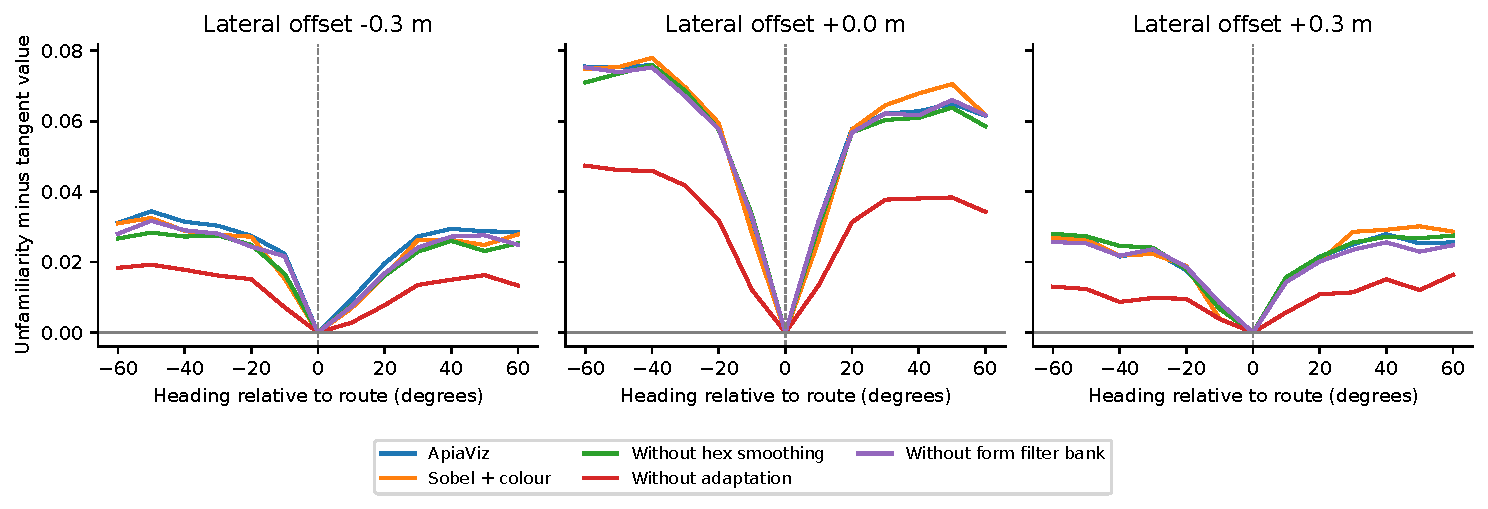
\includegraphics[width=\linewidth]{familiarity.pdf}
\captionof{figure}{\textbf{Recognising the route direction is not sufficient for recovery.}
Lower values are more familiar. Averaged over routes and seeds, familiarity
remains greatest near the tangent even 30\,cm to either side. These averages
can hide individual errors; actual selected turns are summarised below.}
\end{center}

At displaced probes, ApiaViz selected inward, parallel and outward turns
35.5\%, 39.7\% and 24.8\% of the time. Sobel gave 35.1\%, 40.9\% and 24.0\%.
Learning parallel views across a corridor can therefore preserve the forward
direction without supplying a reliable inward correction. This matches a known
limitation of visual-compass navigation~[4]. It is a plausible recovery mechanism,
not proof that the controller alone explains the observed ranking.

\topic{5\quad Implications}
The fixed spiking representation can support navigation, and adaptation clearly
changes the information available to memory. The broader claim that ApiaViz is
a more accurate visual backbone than simple processing is currently unsupported.
The next matched experiment should test route-directed learning and restoring
steering for every frontend, followed by evaluation in independent worlds with
a fixed sample budget. Separately removing the smoothed and ON/OFF channels
would better identify which form computations matter.

All 440 trajectories, 61,091 steering decisions and 35,200 probe decisions
passed reconstruction checks. The faster renderer matched 560 sampled original
images and all four earlier ApiaViz paths and steering scores exactly. These
checks do not replace independent-world validation. Other limits are the five
seeds, previously selected ApiaViz neural settings, and a full template memory
rather than a compact mushroom-body output circuit.

\vspace{3pt}
{\footnotesize
\textbf{Selected references.} Full methods, data, audits and the extended review
accompany this note in \texttt{docs/mechanism-study/}.\\
{}[1] Ardin et al. (2016). \emph{PLoS Comput. Biol.} 12:e1004683.
\href{https://doi.org/10.1371/journal.pcbi.1004683}{doi:10.1371/journal.pcbi.1004683}.\\
{}[2] Gattaux et al. (2025). \emph{Nature Communications}.
\href{https://doi.org/10.1038/s41467-025-62327-3}{doi:10.1038/s41467-025-62327-3}.\\
{}[3] Jesusanmi et al. (2024). \emph{Front. Physiol.} 15:1379977.
\href{https://doi.org/10.3389/fphys.2024.1379977}{doi:10.3389/fphys.2024.1379977}.\\
{}[4] Amin, Philippides \& Graham (2025). \emph{PLoS Comput. Biol.} 21:e1012798.
\href{https://doi.org/10.1371/journal.pcbi.1012798}{doi:10.1371/journal.pcbi.1012798}.\\
{}[5] Owen (2007). The pigeonhole bootstrap. \emph{Ann. Appl. Stat.} 1:386--411.
\href{https://doi.org/10.1214/07-AOAS122}{doi:10.1214/07-AOAS122}.
\par}
\end{document}
